\documentclass[a4paper,zihao=5,UTF8, twoside]{ctexart}

% 基础宏包引用
\usepackage{tikz}
\usepackage{anyfontsize}
\usepackage{framed}
\usepackage{fancybox}
%\usepackage[left=1.25in,right=1.25in,top=1in,bottom=1in]{geometry}
\usepackage[margin=1in]{geometry}
\usepackage{fancyhdr}
\usepackage{amsmath}
\usepackage{graphicx}
\usepackage{float}
\usepackage{caption}
\usepackage{booktabs}
\usepackage{multirow}
\usepackage{hyperref}

\usepackage{color}

% 引用(编译需要使用xe->bib->xe->xe)
\usepackage{cite}
\usepackage{url}


% 如果使用原来的 fancypage fbox 方案会导致tikz 无法绘制于其上
% 所以换用 tikz 方案,这使得可以做一些更诡异的操作
% 缺点是加页面时需要编译多一次
\usepackage{atbegshi}   % 包用于在每页添加元素
\newcommand{\AddFrame}{%
\tikz[overlay,remember picture]{
    \draw
        ([xshift=2.42cm,yshift=-2.42cm]current page.north west)
        rectangle
        ([xshift=-2.42cm,yshift=2.42cm]current page.south east);
    }
}
% 在每页调用 \AddFrame 命令
\AtBeginShipout{\AtBeginShipoutAddToBox{\AddFrame}}


% section 设置
\usepackage{zhnumber} 
\usepackage{titlesec}
\titleformat{\section}[block]{\bfseries\normalsize}{\hspace{3pt}\zhnum{section}、}{0em}{}[\texorpdfstring{\noindent\begin{tikzpicture}[overlay]
   \draw (-0.115,0.3) -- (16.03,0.3); 
   \draw (-0.115,1.15) -- (16.03,1.15); 
  \end{tikzpicture}\begin{tikzpicture}[remember picture,overlay]
			\node[anchor=north, fill=white, minimum width=\paperwidth, minimum height=1in] at (current page.north) {};
		\end{tikzpicture}}]

\titleformat{\subsection}[block]{\normalfont\normalsize}{\arabic{subsection}. }{0em}{}
\titleformat{\subsubsection}[block]{\normalfont\normalsize}{\hspace{2em} \arabic{subsubsection}. }{0em}{}


% 表格中使用 C 即1cm宽的空表
\usepackage{comment}
\usepackage{array}
\newcolumntype{C}{>{\centering\arraybackslash}m{1.0cm}}

% 图表标题字样小一号
\captionsetup{font={small}}


% 每章节之间的分割符定义
\NewDocumentCommand\tableSearator{}
{
  \noindent\begin{tikzpicture}[overlay]
   \draw (-0.12,-0) -- (16.03,-0.2); 
  \end{tikzpicture}
}


\newcommand{\dif}{\mathrm{d}}

% 版面设置
\pagestyle{fancy}
\lhead{}
\chead{}
\rhead{}
\lfoot{}
\cfoot{}
\rfoot{\thepage}
\renewcommand{\headrulewidth}{0pt} % 页眉线宽设为0,即不显示页眉线

\date{\today}
\begin{document}

\section{选题意义}

\quad\vspace{2cm}

\noindent\begin{tikzpicture}[overlay]
  \filldraw[white] (-5, 2.15) rectangle (20, 20);
  \draw (-0.12,1.4) -- (16.03,1.4);
  \draw (-0.12,2.15) -- (16.03,2.15);
  \draw (-0.12,0.65) -- (16.03,0.65);
  \node[right] at (0, 0.25) {\textbf{一、选题意义}};
  \draw (-0.12,-0.1) -- (16.03,-0.1);
  \node[font=\huge] at (\linewidth * 0.5, 3.2) {\textbf{大学物理实验三设计性实验调研报告}};

  \draw (1.8, 2.15) -- (1.8, 0.65);
  \draw (7, 2.15) -- (7, 1.4);
  \draw (8, 2.15) -- (8, 1.4);
  \draw (11, 2.15) -- (11, 1.4);
  \draw (12, 2.15) -- (12, 1.4);

  %
  %%以下需要修改%%
  %
  \node[right] at (0, 1.775) {\textbf{课程编号}};
  \node[right] at (0, 1.025) {\textbf{实验名称}};

  \node[right] at (1.8, 1.775) {(课程编号)};
  \node[right] at (1.8, 1.025) {(实验名称)};

  \node[right] at (7, 1.775) {\textbf{组号}};
  \node[right] at (8, 1.775) {(组号)};

  \node[right] at (11, 1.775) {\textbf{姓名}};
  \node[right] at (12, 1.775) {(姓名)};
  %
  %%%%%%%%%%%%%%
  %

\end{tikzpicture}

选题意义部分

\section{文献归纳}

内容

\subsection{子章节}

\subsection{子章节2}

%\nocite{*}
%\bibliographystyle{unsrt}
%\bibliography{ref.bib}

\section{预期目标}

简述拟采用何种方法,通过实验解决什么问题?达到什么目标?


【预期目标举例】

通过分析目前光电计时法测量转动惯量中所存在的问题,提出一种基于阻尼比实时算法,利用计算的阻尼比对转动惯量测量值进行实时修正,实现转动惯量的高精度测量。


\section{指导教师意见}

\vspace{4cm}

\noindent\begin{tikzpicture}[overlay]
  \draw (-0.12,0.6) -- (16.03,0.6);
  \node[right] at (0.1, 0.25) {成绩 \hspace{4cm} 签章: \hspace{5cm} 年 \hspace{1cm} 月 \hspace{1cm} 日};
  \filldraw[white] (-5, -0.2) rectangle (30, -50);
  \draw (-0.12,-0.2) -- (16.03,-0.2);
\end{tikzpicture}

\end{document}
